%\section{appendix}
\label{sec:tables}




\vspace{30 mm}
\begin{figure}[htb]
\begin{center}
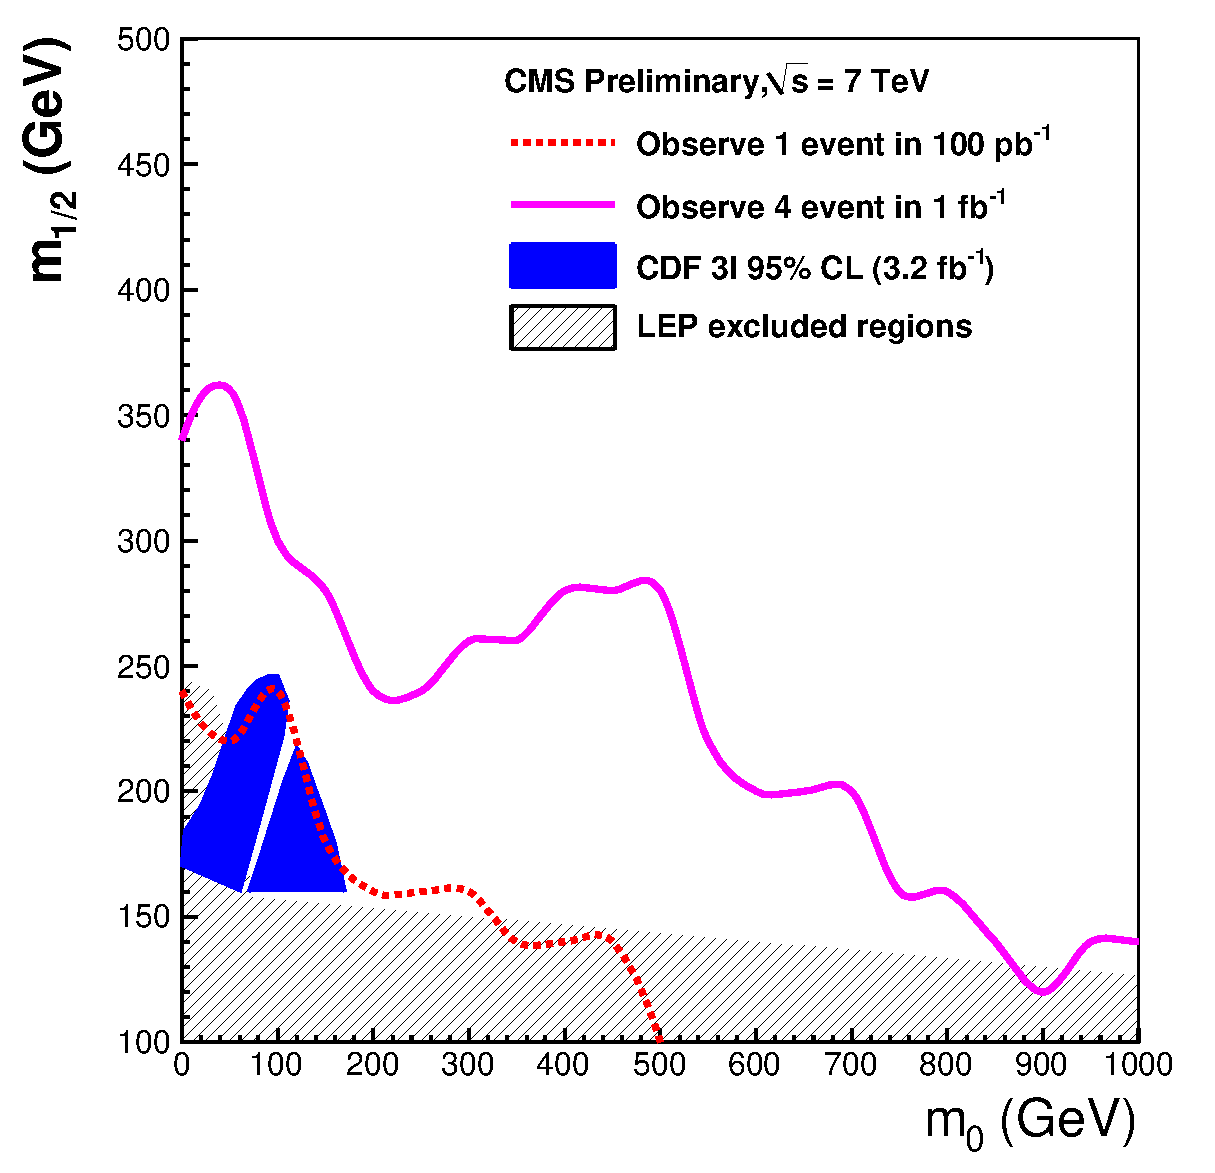
\includegraphics[width=0.7\linewidth]{figs/exclusion1fbssa.eps}
\caption{The $m_{0}-m_{1/2}$ exclusion plot at the 95\% CL in the framework of
mSUGRA assuming R-parity conservation using an  integrated  luminosity of
$100~\mathrm{pb}^{-1}$ and $1~\mathrm{fb}^{-1}$. The solid regions (blue/green) were
excluded by the Tevatron (CDF/D0) experiments~\cite{cdf:recentSusy, d0:recentSusy}.
The black hashed region was excluded by the LEP experiments~\cite{lep:lepsusyreach}.
\label{fig:ssadd_exclusion}}

\end{center}
\end{figure}


\begin{table}[hbt]
\begin{center}
\renewcommand{\arraystretch}{2.0}
 {\footnotesize
\begin{tabular}{|l|c|c|c|c|c|c|c|c|}\hline
$m_{0}$ GeV & $m_{1/2}$ GeV & Event Yield & Raw Event Yield \\ \hline
0 & 240.0 & 5.2 $\pm$ 0.6 & 84.0 $\pm$ 9.2 \\ 
50 & 240.0 & 3.3 $\pm$ 0.4 & 56.0 $\pm$ 7.5 \\ 
100 & 260.0 & 4.7 $\pm$ 0.4 & 130.0 $\pm$ 11.4 \\ 
150 & 260.0 & 4.6 $\pm$ 0.4 & 139.0 $\pm$ 11.8 \\ 
200 & 200.0 & 3.6 $\pm$ 0.7 & 30.0 $\pm$ 5.5 \\ 
250 & 180.0 & 4.1 $\pm$ 0.8 & 24.0 $\pm$ 4.9 \\ 
300 & 180.0 & 4.6 $\pm$ 0.8 & 32.0 $\pm$ 5.7 \\ 
350 & 200.0 & 3.4 $\pm$ 0.5 & 45.0 $\pm$ 6.7 \\ 
400 & 140.0 & 10.3 $\pm$ 1.8 & 31.0 $\pm$ 5.6 \\ \hline
\end{tabular} }
\caption{Expected weighted and raw event yields in mSUGRA $m_{0}-m_{1/2}$ plane with tan$\beta = 3$, A$_0 = 0$, $\mu > 0$. The weighted yields are normalized to 100 pb$^{-1}$ of integrated luminosity and are used in case of 0 observed event hypothesis. Uncertainties are from MC statistics. \label{tab:ssyields_ex0}}
\end{center}
\end{table}

\vspace{10 mm}
\begin{table}[hbt]
\begin{center}
\renewcommand{\arraystretch}{2.0}
 {\footnotesize
\begin{tabular}{|l|c|c|c|c|c|c|c|c|}\hline
$m_{0}$ GeV & $m_{1/2}$ GeV & Event Yield & Raw Event Yield \\ \hline
0 & 240.0 & 5.2 $\pm$ 0.6 & 84.0 $\pm$ 9.2 \\ 
50 & 220.0 & 6.5 $\pm$ 0.8 & 68.0 $\pm$ 8.2 \\ 
100 & 240.0 & 6.6 $\pm$ 0.6 & 117.0 $\pm$ 10.8 \\ 
150 & 180.0 & 9.7 $\pm$ 1.5 & 42.0 $\pm$ 6.5 \\ 
200 & 160.0 & 10.3 $\pm$ 1.9 & 29.0 $\pm$ 5.4 \\ 
250 & 160.0 & 8.4 $\pm$ 1.6 & 28.0 $\pm$ 5.3 \\ 
300 & 160.0 & 6.5 $\pm$ 1.3 & 26.0 $\pm$ 5.1 \\ 
350 & 140.0 & 7.8 $\pm$ 1.8 & 20.0 $\pm$ 4.5 \\ 
400 & 140.0 & 10.3 $\pm$ 1.8 & 31.0 $\pm$ 5.6 \\ 
450 & 140.0 & 10.1 $\pm$ 1.7 & 36.0 $\pm$ 6.0 \\ 
500 & 100.0 & 6.8 $\pm$ 3.1 & 5.0 $\pm$ 2.2 \\ \hline
\end{tabular} }
\caption{Expected weighted and raw event yields in mSUGRA $m_{0}-m_{1/2}$ plane with tan$\beta = 3$, A$_0 = 0$, $\mu > 0$. The weighted yields are normalized to 100 pb$^{-1}$ of integrated luminosity and are used in case of 1 observed event hypothesis. Uncertainties are from MC statistics. \label{tab:ssyields_ex1}}
\end{center}
\end{table}

\vspace{10 mm}
\begin{table}[hbt]
\begin{center}
\renewcommand{\arraystretch}{2.0}
 {\footnotesize
\begin{tabular}{|l|c|c|c|c|c|c|c|c|}\hline
$m_{0}$ GeV & $m_{1/2}$ GeV & Event Yield & Raw Event Yield \\ \hline
0 & 340.0 & 10.9 $\pm$ 0.1 & 132.0 $\pm$ 11.5 \\ 
50 & 360.0 & 7.4 $\pm$ 0.1 & 130.0 $\pm$ 11.4 \\ 
100 & 300.0 & 10.4 $\pm$ 0.1 & 66.0 $\pm$ 8.1 \\ 
150 & 280.0 & 20.6 $\pm$ 0.2 & 95.0 $\pm$ 9.7 \\ 
200 & 240.0 & 14.3 $\pm$ 0.3 & 31.0 $\pm$ 5.6 \\ 
250 & 240.0 & 7.8 $\pm$ 0.2 & 19.0 $\pm$ 4.4 \\ 
300 & 260.0 & 7.6 $\pm$ 0.1 & 32.0 $\pm$ 5.7 \\ 
350 & 260.0 & 7.6 $\pm$ 0.1 & 36.0 $\pm$ 6.0 \\ 
400 & 280.0 & 8.8 $\pm$ 0.1 & 70.0 $\pm$ 8.4 \\ 
450 & 280.0 & 9.6 $\pm$ 0.1 & 86.0 $\pm$ 9.3 \\ 
500 & 280.0 & 8.0 $\pm$ 0.1 & 82.0 $\pm$ 9.1 \\ 
550 & 220.0 & 10.1 $\pm$ 0.2 & 36.0 $\pm$ 6.0 \\ 
600 & 200.0 & 10.8 $\pm$ 0.2 & 28.0 $\pm$ 5.3 \\ 
650 & 200.0 & 11.3 $\pm$ 0.2 & 32.0 $\pm$ 5.7 \\ 
700 & 200.0 & 10.0 $\pm$ 0.2 & 31.0 $\pm$ 5.6 \\ 
750 & 160.0 & 9.4 $\pm$ 0.3 & 11.0 $\pm$ 3.3 \\ 
800 & 160.0 & 8.0 $\pm$ 0.3 & 10.0 $\pm$ 3.2 \\ 
850 & 140.0 & 8.8 $\pm$ 0.4 & 6.0 $\pm$ 2.4 \\ 
900 & 120.0 & 12.2 $\pm$ 0.6 & 4.0 $\pm$ 2.0 \\ 
950 & 140.0 & 15.0 $\pm$ 0.5 & 11.0 $\pm$ 3.3 \\ 
1000 & 140.0 & 10.7 $\pm$ 0.4 & 8.0 $\pm$ 2.8 \\ \hline
\end{tabular} }
\caption{Expected weighted and raw event yields in mSUGRA $m_{0}-m_{1/2}$ plane with tan$\beta = 3$, A$_0 = 0$, $\mu > 0$. The weighted yields are normalized to 1 fb$^{-1}$ of integrated luminosity and are used in case of 4 observed event hypothesis. Uncertainties are from MC statistics. \label{tab:ssyields_ex1fb}}
\end{center}
\end{table}
